\documentclass{standalone}
\usepackage{tikz}
\usetikzlibrary{patterns, positioning}

\begin{document}
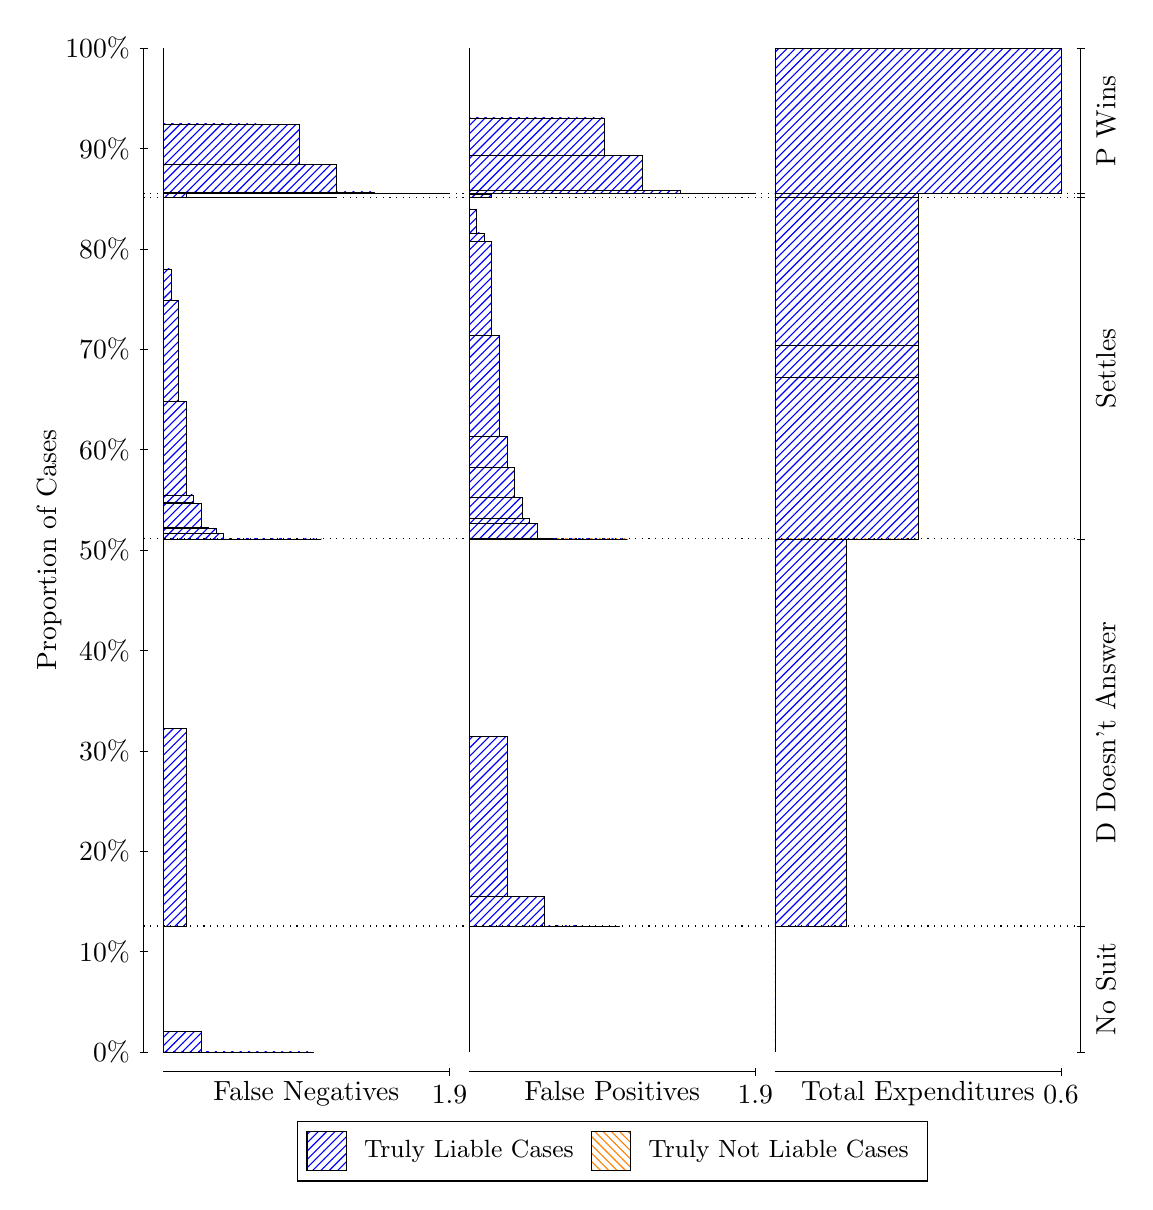
\begin{tikzpicture}
\draw[black, very thin] (1.5,1.75) -- (1.5,14.5);
\node[rotate=90, anchor=center] at (0.3, 8.125) {Proportion of Cases};
\draw[black, very thin] (1.45,1.75) -- (1.55,1.75);
\node[anchor=east] at (1.45, 1.75) {0\%};
\draw[black, very thin] (1.45,3.025) -- (1.55,3.025);
\node[anchor=east] at (1.45, 3.025) {10\%};
\draw[black, very thin] (1.45,4.3) -- (1.55,4.3);
\node[anchor=east] at (1.45, 4.3) {20\%};
\draw[black, very thin] (1.45,5.575) -- (1.55,5.575);
\node[anchor=east] at (1.45, 5.575) {30\%};
\draw[black, very thin] (1.45,6.85) -- (1.55,6.85);
\node[anchor=east] at (1.45, 6.85) {40\%};
\draw[black, very thin] (1.45,8.125) -- (1.55,8.125);
\node[anchor=east] at (1.45, 8.125) {50\%};
\draw[black, very thin] (1.45,9.4) -- (1.55,9.4);
\node[anchor=east] at (1.45, 9.4) {60\%};
\draw[black, very thin] (1.45,10.675) -- (1.55,10.675);
\node[anchor=east] at (1.45, 10.675) {70\%};
\draw[black, very thin] (1.45,11.95) -- (1.55,11.95);
\node[anchor=east] at (1.45, 11.95) {80\%};
\draw[black, very thin] (1.45,13.225) -- (1.55,13.225);
\node[anchor=east] at (1.45, 13.225) {90\%};
\draw[black, very thin] (1.45,14.5) -- (1.55,14.5);
\node[anchor=east] at (1.45, 14.5) {100\%};

\draw[black, very thin] (13.4,1.75) -- (13.4,14.5);
\draw[black, very thin] (13.35,1.75) -- (13.45,1.75);
\node[anchor=west] at (13.35, 1.75) {};
\draw[black, very thin] (13.35,3.3493) -- (13.45,3.3493);
\node[anchor=west] at (13.35, 3.3493) {};
\draw[black, very thin] (13.35,8.2665) -- (13.45,8.2665);
\node[anchor=west] at (13.35, 8.2665) {};
\draw[black, very thin] (13.35,12.602) -- (13.45,12.602);
\node[anchor=west] at (13.35, 12.602) {};
\draw[black, very thin] (13.35,12.651) -- (13.45,12.651);
\node[anchor=west] at (13.35, 12.651) {};
\draw[black, very thin] (13.35,14.5) -- (13.45,14.5);
\node[anchor=west] at (13.35, 14.5) {};

\draw[black, very thin, pattern color=blue, pattern=north east lines] (1.75,1.75) rectangle (3.6623,1.75);
\draw[black, very thin, pattern color=blue, pattern=north east lines] (1.75,1.75) rectangle (3.1842,1.75);
\draw[black, very thin, pattern color=blue, pattern=north east lines] (1.75,1.75) rectangle (2.7061,1.7522);
\draw[black, very thin, pattern color=blue, pattern=north east lines] (1.75,1.7522) rectangle (2.2281,2.0119);
\draw[black, very thin, pattern color=orange, pattern=north west lines] (1.75,2.0119) rectangle (1.75,2.0119);
\draw[black, very thin, pattern color=blue, pattern=north east lines] (1.75,2.0119) rectangle (1.75,3.3493);
\draw[black, very thin, pattern color=blue, pattern=north east lines] (1.75,3.3493) rectangle (2.0368,5.8622);
\draw[black, very thin, pattern color=orange, pattern=north west lines] (1.75,5.8622) rectangle (1.75,5.8622);
\draw[black, very thin, pattern color=blue, pattern=north east lines] (1.75,5.8622) rectangle (1.75,8.2665);
\draw[black, very thin, pattern color=blue, pattern=north east lines] (1.75,8.2665) rectangle (3.7579,8.2665);
\draw[black, very thin, pattern color=blue, pattern=north east lines] (1.75,8.2665) rectangle (3.5667,8.2665);
\draw[black, very thin, pattern color=blue, pattern=north east lines] (1.75,8.2665) rectangle (3.3754,8.2665);
\draw[black, very thin, pattern color=blue, pattern=north east lines] (1.75,8.2665) rectangle (3.2798,8.2665);
\draw[black, very thin, pattern color=blue, pattern=north east lines] (1.75,8.2665) rectangle (3.1842,8.2665);
\draw[black, very thin, pattern color=blue, pattern=north east lines] (1.75,8.2665) rectangle (3.0886,8.2665);
\draw[black, very thin, pattern color=blue, pattern=north east lines] (1.75,8.2665) rectangle (2.993,8.2665);
\draw[black, very thin, pattern color=blue, pattern=north east lines] (1.75,8.2665) rectangle (2.8974,8.2665);
\draw[black, very thin, pattern color=blue, pattern=north east lines] (1.75,8.2665) rectangle (2.8018,8.2665);
\draw[black, very thin, pattern color=blue, pattern=north east lines] (1.75,8.2665) rectangle (2.7061,8.267);
\draw[black, very thin, pattern color=blue, pattern=north east lines] (1.75,8.267) rectangle (2.6105,8.2671);
\draw[black, very thin, pattern color=blue, pattern=north east lines] (1.75,8.2671) rectangle (2.6105,8.2672);
\draw[black, very thin, pattern color=blue, pattern=north east lines] (1.75,8.2672) rectangle (2.5149,8.3313);
\draw[black, very thin, pattern color=blue, pattern=north east lines] (1.75,8.3313) rectangle (2.4193,8.3952);
\draw[black, very thin, pattern color=blue, pattern=north east lines] (1.75,8.3952) rectangle (2.3237,8.3954);
\draw[black, very thin, pattern color=blue, pattern=north east lines] (1.75,8.3954) rectangle (2.3237,8.4103);
\draw[black, very thin, pattern color=blue, pattern=north east lines] (1.75,8.4103) rectangle (2.2281,8.7169);
\draw[black, very thin, pattern color=blue, pattern=north east lines] (1.75,8.7169) rectangle (2.1325,8.7361);
\draw[black, very thin, pattern color=blue, pattern=north east lines] (1.75,8.7361) rectangle (2.1325,8.8263);
\draw[black, very thin, pattern color=blue, pattern=north east lines] (1.75,8.8263) rectangle (2.0368,10.016);
\draw[black, very thin, pattern color=blue, pattern=north east lines] (1.75,10.016) rectangle (1.9412,11.297);
\draw[black, very thin, pattern color=blue, pattern=north east lines] (1.75,11.297) rectangle (1.9412,11.297);
\draw[black, very thin, pattern color=blue, pattern=north east lines] (1.75,11.297) rectangle (1.8456,11.302);
\draw[black, very thin, pattern color=blue, pattern=north east lines] (1.75,11.302) rectangle (1.8456,11.696);
\draw[black, very thin, pattern color=orange, pattern=north west lines] (1.75,11.696) rectangle (1.75,11.696);
\draw[black, very thin, pattern color=blue, pattern=north east lines] (1.75,11.696) rectangle (1.75,12.602);
\draw[black, very thin, pattern color=blue, pattern=north east lines] (1.75,12.602) rectangle (3.9491,12.602);
\draw[black, very thin, pattern color=blue, pattern=north east lines] (1.75,12.602) rectangle (3.4711,12.602);
\draw[black, very thin, pattern color=blue, pattern=north east lines] (1.75,12.602) rectangle (2.993,12.602);
\draw[black, very thin, pattern color=blue, pattern=north east lines] (1.75,12.602) rectangle (2.5149,12.608);
\draw[black, very thin, pattern color=blue, pattern=north east lines] (1.75,12.608) rectangle (2.0368,12.651);
\draw[black, very thin, pattern color=orange, pattern=north west lines] (1.75,12.651) rectangle (1.75,12.651);
\draw[black, very thin, pattern color=blue, pattern=north east lines] (1.75,12.651) rectangle (5.3833,12.651);
\draw[black, very thin, pattern color=blue, pattern=north east lines] (1.75,12.651) rectangle (4.9053,12.651);
\draw[black, very thin, pattern color=blue, pattern=north east lines] (1.75,12.651) rectangle (4.4272,12.673);
\draw[black, very thin, pattern color=blue, pattern=north east lines] (1.75,12.673) rectangle (3.9491,13.023);
\draw[black, very thin, pattern color=blue, pattern=north east lines] (1.75,13.023) rectangle (3.4711,13.532);
\draw[black, very thin, pattern color=blue, pattern=north east lines] (1.75,13.532) rectangle (2.993,13.536);
\draw[black, very thin, pattern color=blue, pattern=north east lines] (1.75,13.536) rectangle (2.6105,13.536);
\draw[black, very thin, pattern color=blue, pattern=north east lines] (1.75,13.536) rectangle (2.5149,13.536);
\draw[black, very thin, pattern color=blue, pattern=north east lines] (1.75,13.536) rectangle (2.1325,13.536);
\draw[black, very thin, pattern color=orange, pattern=north west lines] (1.75,13.536) rectangle (1.75,13.536);
\draw[black, very thin, pattern color=blue, pattern=north east lines] (1.75,13.536) rectangle (1.75,14.5);
\draw[black, very thin, pattern color=orange, pattern=north west lines] (5.6333,1.75) rectangle (5.6333,1.75);
\draw[black, very thin, pattern color=blue, pattern=north east lines] (5.6333,1.75) rectangle (5.6333,3.3493);
\draw[black, very thin, pattern color=orange, pattern=north west lines] (5.6333,3.3493) rectangle (7.5456,3.3493);
\draw[black, very thin, pattern color=blue, pattern=north east lines] (5.6333,3.3493) rectangle (7.5456,3.3493);
\draw[black, very thin, pattern color=blue, pattern=north east lines] (5.6333,3.3493) rectangle (7.0675,3.3522);
\draw[black, very thin, pattern color=blue, pattern=north east lines] (5.6333,3.3522) rectangle (6.5895,3.7288);
\draw[black, very thin, pattern color=blue, pattern=north east lines] (5.6333,3.7288) rectangle (6.1114,5.7535);
\draw[black, very thin, pattern color=blue, pattern=north east lines] (5.6333,5.7535) rectangle (5.6333,8.2665);
\draw[black, very thin, pattern color=orange, pattern=north west lines] (5.6333,8.2665) rectangle (7.6412,8.2665);
\draw[black, very thin, pattern color=blue, pattern=north east lines] (5.6333,8.2665) rectangle (7.6412,8.2665);
\draw[black, very thin, pattern color=orange, pattern=north west lines] (5.6333,8.2665) rectangle (7.45,8.2665);
\draw[black, very thin, pattern color=blue, pattern=north east lines] (5.6333,8.2665) rectangle (7.45,8.2665);
\draw[black, very thin, pattern color=orange, pattern=north west lines] (5.6333,8.2665) rectangle (7.2588,8.2665);
\draw[black, very thin, pattern color=blue, pattern=north east lines] (5.6333,8.2665) rectangle (7.2588,8.2665);
\draw[black, very thin, pattern color=blue, pattern=north east lines] (5.6333,8.2665) rectangle (7.1632,8.2665);
\draw[black, very thin, pattern color=orange, pattern=north west lines] (5.6333,8.2665) rectangle (7.0675,8.2665);
\draw[black, very thin, pattern color=blue, pattern=north east lines] (5.6333,8.2665) rectangle (7.0675,8.2665);
\draw[black, very thin, pattern color=blue, pattern=north east lines] (5.6333,8.2665) rectangle (6.9719,8.2665);
\draw[black, very thin, pattern color=orange, pattern=north west lines] (5.6333,8.2665) rectangle (6.8763,8.2665);
\draw[black, very thin, pattern color=blue, pattern=north east lines] (5.6333,8.2665) rectangle (6.8763,8.2665);
\draw[black, very thin, pattern color=blue, pattern=north east lines] (5.6333,8.2665) rectangle (6.7807,8.2665);
\draw[black, very thin, pattern color=orange, pattern=north west lines] (5.6333,8.2665) rectangle (6.6851,8.2665);
\draw[black, very thin, pattern color=blue, pattern=north east lines] (5.6333,8.2665) rectangle (6.6851,8.2717);
\draw[black, very thin, pattern color=blue, pattern=north east lines] (5.6333,8.2717) rectangle (6.5895,8.2719);
\draw[black, very thin, pattern color=blue, pattern=north east lines] (5.6333,8.2719) rectangle (6.4939,8.2719);
\draw[black, very thin, pattern color=orange, pattern=north west lines] (5.6333,8.2719) rectangle (6.4939,8.2719);
\draw[black, very thin, pattern color=blue, pattern=north east lines] (5.6333,8.2719) rectangle (6.4939,8.4652);
\draw[black, very thin, pattern color=blue, pattern=north east lines] (5.6333,8.4652) rectangle (6.3982,8.5291);
\draw[black, very thin, pattern color=orange, pattern=north west lines] (5.6333,8.5291) rectangle (6.3026,8.5291);
\draw[black, very thin, pattern color=blue, pattern=north east lines] (5.6333,8.5291) rectangle (6.3026,8.7964);
\draw[black, very thin, pattern color=blue, pattern=north east lines] (5.6333,8.7964) rectangle (6.207,9.1725);
\draw[black, very thin, pattern color=orange, pattern=north west lines] (5.6333,9.1725) rectangle (6.1114,9.1725);
\draw[black, very thin, pattern color=blue, pattern=north east lines] (5.6333,9.1725) rectangle (6.1114,9.5708);
\draw[black, very thin, pattern color=blue, pattern=north east lines] (5.6333,9.5708) rectangle (6.0158,9.5708);
\draw[black, very thin, pattern color=blue, pattern=north east lines] (5.6333,9.5708) rectangle (6.0158,10.853);
\draw[black, very thin, pattern color=blue, pattern=north east lines] (5.6333,10.853) rectangle (5.9202,12.042);
\draw[black, very thin, pattern color=blue, pattern=north east lines] (5.6333,12.042) rectangle (5.8246,12.151);
\draw[black, very thin, pattern color=blue, pattern=north east lines] (5.6333,12.151) rectangle (5.7289,12.458);
\draw[black, very thin, pattern color=blue, pattern=north east lines] (5.6333,12.458) rectangle (5.6333,12.602);
\draw[black, very thin, pattern color=orange, pattern=north west lines] (5.6333,12.602) rectangle (5.9202,12.602);
\draw[black, very thin, pattern color=blue, pattern=north east lines] (5.6333,12.602) rectangle (5.9202,12.644);
\draw[black, very thin, pattern color=blue, pattern=north east lines] (5.6333,12.644) rectangle (5.6333,12.651);
\draw[black, very thin, pattern color=orange, pattern=north west lines] (5.6333,12.651) rectangle (9.2667,12.651);
\draw[black, very thin, pattern color=blue, pattern=north east lines] (5.6333,12.651) rectangle (9.2667,12.651);
\draw[black, very thin, pattern color=orange, pattern=north west lines] (5.6333,12.651) rectangle (8.7886,12.651);
\draw[black, very thin, pattern color=blue, pattern=north east lines] (5.6333,12.651) rectangle (8.7886,12.651);
\draw[black, very thin, pattern color=orange, pattern=north west lines] (5.6333,12.651) rectangle (8.3105,12.651);
\draw[black, very thin, pattern color=blue, pattern=north east lines] (5.6333,12.651) rectangle (8.3105,12.688);
\draw[black, very thin, pattern color=orange, pattern=north west lines] (5.6333,12.688) rectangle (7.8325,12.688);
\draw[black, very thin, pattern color=blue, pattern=north east lines] (5.6333,12.688) rectangle (7.8325,13.138);
\draw[black, very thin, pattern color=blue, pattern=north east lines] (5.6333,13.138) rectangle (7.3544,13.612);
\draw[black, very thin, pattern color=blue, pattern=north east lines] (5.6333,13.612) rectangle (6.8763,13.614);
\draw[black, very thin, pattern color=blue, pattern=north east lines] (5.6333,13.614) rectangle (6.3982,13.614);
\draw[black, very thin, pattern color=orange, pattern=north west lines] (5.6333,13.614) rectangle (6.0158,13.614);
\draw[black, very thin, pattern color=blue, pattern=north east lines] (5.6333,13.614) rectangle (6.0158,13.614);
\draw[black, very thin, pattern color=blue, pattern=north east lines] (5.6333,13.614) rectangle (5.9202,13.614);
\draw[black, very thin, pattern color=orange, pattern=north west lines] (5.6333,13.614) rectangle (5.6333,13.614);
\draw[black, very thin, pattern color=blue, pattern=north east lines] (5.6333,13.614) rectangle (5.6333,14.5);
\draw[black, very thin, pattern color=orange, pattern=north west lines] (9.5167,1.75) rectangle (9.5167,1.75);
\draw[black, very thin, pattern color=blue, pattern=north east lines] (9.5167,1.75) rectangle (9.5167,3.3493);
\draw[black, very thin, pattern color=orange, pattern=north west lines] (9.5167,3.3493) rectangle (10.425,3.3493);
\draw[black, very thin, pattern color=blue, pattern=north east lines] (9.5167,3.3493) rectangle (10.425,8.2665);
\draw[black, very thin, pattern color=orange, pattern=north west lines] (9.5167,8.2665) rectangle (11.333,8.2665);
\draw[black, very thin, pattern color=blue, pattern=north east lines] (9.5167,8.2665) rectangle (11.333,10.315);
\draw[black, very thin, pattern color=orange, pattern=north west lines] (9.5167,10.315) rectangle (11.333,10.315);
\draw[black, very thin, pattern color=blue, pattern=north east lines] (9.5167,10.315) rectangle (11.333,10.724);
\draw[black, very thin, pattern color=orange, pattern=north west lines] (9.5167,10.724) rectangle (11.333,10.724);
\draw[black, very thin, pattern color=blue, pattern=north east lines] (9.5167,10.724) rectangle (11.333,12.602);
\draw[black, very thin, pattern color=orange, pattern=north west lines] (9.5167,12.602) rectangle (11.333,12.602);
\draw[black, very thin, pattern color=blue, pattern=north east lines] (9.5167,12.602) rectangle (11.333,12.651);
\draw[black, very thin, pattern color=orange, pattern=north west lines] (9.5167,12.651) rectangle (13.15,12.651);
\draw[black, very thin, pattern color=blue, pattern=north east lines] (9.5167,12.651) rectangle (13.15,14.5);
\draw[black, dotted] (1.5,3.3493) -- (13.4,3.3493);
\draw[black, dotted] (1.5,8.2665) -- (13.4,8.2665);
\draw[black, dotted] (1.5,12.602) -- (13.4,12.602);
\draw[black, dotted] (1.5,12.651) -- (13.4,12.651);
\draw[black, very thin] (1.75,1.5) -- (5.3833,1.5);
\node[anchor=north] at (3.5667, 1.5) {False Negatives};
\draw[black, very thin] (5.3833,1.45) -- (5.3833,1.55);
\node[anchor=north] at (5.3833, 1.45) {1.9};

\draw[black, very thin] (5.6333,1.5) -- (9.2667,1.5);
\node[anchor=north] at (7.45, 1.5) {False Positives};
\draw[black, very thin] (9.2667,1.45) -- (9.2667,1.55);
\node[anchor=north] at (9.2667, 1.45) {1.9};

\draw[black, very thin] (9.5167,1.5) -- (13.15,1.5);
\node[anchor=north] at (11.333, 1.5) {Total Expenditures};
\draw[black, very thin] (13.15,1.45) -- (13.15,1.55);
\node[anchor=north] at (13.15, 1.45) {0.6};

\node[black, centered, rotate=90] at (13.72, 2.5496) {No Suit};
\node[black, centered, rotate=90] at (13.72, 5.8079) {D Doesn't Answer};
\node[black, centered, rotate=90] at (13.72, 10.434) {Settles};

\node[black, centered, rotate=90] at (13.72, 13.575) {P Wins};

\draw (7.449999999999999,1.5) node[draw=none] (baseCoordinate) {};
\begin{scope}[align=center]
        \matrix[scale=0.5, draw=black, below=0.5cm of baseCoordinate, nodes={draw}, column sep=0.1cm]{
            \node[rectangle, draw, minimum width=0.5cm, minimum height=0.5cm, pattern=north east lines, pattern color=blue] {}; &
            \node[draw=none, font=\small] (B) {Truly Liable Cases}; &
            \node[rectangle, draw, minimum width=0.5cm, minimum height=0.5cm, pattern=north west lines, pattern color=orange] {}; &
            \node[draw=none, font=\small] (B) {Truly Not Liable Cases}; \\
            };
\end{scope}

\end{tikzpicture}
\end{document}